\newif\ifJPN
\JPNtrue
\JPNfalse
\ifJPN
  \documentclass[a4paper,xelatex,ja=standard]{bxjsarticle}
\else
  \documentclass[a4paper,xelatex,english,ja=standard]{bxjsarticle}
\fi

%\setCJKmainfont[BoldFont=HaranoAjiMincho-Bold.otf]{HaranoAjiMincho-Regular.otf}
%\setCJKsansfont[BoldFont=HaranoAjiGothic-Bold.otf]{HaranoAjiGothic-Regular.otf}
\setCJKmonofont[BoldFont=HaranoAjiGothic-Bold.otf]{HaranoAjiGothic-Regular.otf}

\ifJPN
\usepackage[backend=biber,style=authoryear]{biblatex-japanese} % BibLaTeX と Biber 
\DeclareLanguageMapping{japanese}{japanese}
\else
\usepackage[backend=biber,style=authoryear]{biblatex} % BibLaTeX と Biber を使用
\fi
\addbibresource{koten.bib} % BibTeX ファイルを指定
\usepackage{enumitem}
\usepackage{tikz}
\usetikzlibrary{arrows.meta, positioning}

\usetikzlibrary{positioning}
\usepackage{version}
\usepackage{amssymb}
\usepackage{amsmath}
\usepackage{booktabs} % このパッケージを追加
\usepackage{graphicx}
\usepackage{standalone}
\usepackage{url}
\usepackage{makeidx}
\usepackage{silence}
\WarningFilter{latexfont}{Font shape}
\WarningFilter{latexfont}{Some font shapes}
\WarningFilter{natbib}{There were undefined citations}
\WarningFilter{natbib}{Package natbib Warning}
\usepackage{metalogo} % \XeLaTeX ロゴのため
\usepackage{fancyvrb}
\usepackage{color}
\usepackage{amsmath}
\usepackage{listings} % シンプルで効果的なコードリスト表示
\lstset{
  language=Python,         % Pythonのシンタックスハイライト
  frame=t,            % 全体を枠線で囲む
  basicstyle=\ttfamily\footnotesize, % コードのフォントe定
  numbers=left,            % 行番号を左に表示
  numberstyle=\tiny,       % 行番号のフォントを小さくする
  stepnumber=1,            % 行番号を1行ごとに表示
  tabsize=4,               % タブのサイズを指定
  breaklines=true,         % 長い行を自動的に折り返す
  showstringspaces=false,  % 文字列の空白を表示しない
  keywordstyle=\color{blue}, % キーワードに色を付ける
  commentstyle=\color{black}, % コメントに色を付ける
  stringstyle=\color{red}, % 文字列に色を付ける
}
\usepackage{layout}
%\usepackage{natbib}
\usepackage{support-caption}
\usepackage[format=hang,labelsep=colon,margin=10pt,sc,normalsize]{caption}
%\captionsetup[table]{skip=0pt}
%\captionsetup[figure]{skip=10pt}
%\bibpunct[:\,]{(}{)}{,}{a}{}

\usepackage{hyperref}
\usepackage{url}
\usepackage{makeidx}



\makeindex

\ifJPN
%\captionsetup[table]{name=表}
%\captionsetup[figure]{name=図}
\renewcommand{\refname}{文献}
\renewcommand{\indexname}{索引}
\else
%\captionsetup[table]{name=Table~}
%\captionsetup[figure]{name=Figure~}
\renewcommand{\refname}{Reference}
\renewcommand{\indexname}{Index}
\fi

\if0
\newcounter{marginparcnt}[chapter]
\newcommand{\theMarginparcnt}{$\dagger$\arabic{marginparcnt}}
\newcommand{\Marginpar}[2][-7pt]{%
  \stepcounter{marginparcnt}%
  \textcolor{red}{\textsuperscript{\theMarginparcnt}}%
  \protect\marginpar{\vskip#1\footnotesize\color{blue}%
    \textsuperscript{\theMarginparcnt}
    {#2}\par}}
  \fi

\ifJPN
\title{プロセス文法モデル\\即時文法と調整文法}
\author{
  山元 啓史\\東京科学大学
%\and
%  \Large\textbf{ホドシチェク ボル}\\\Large\textbf{大阪大学}
}
\else
\title{Process Grammar Model\\Immediate Grammar and Adjustive Grammar}
\author{
Hilofumi Yamamoto\\Institute of Science Tokyo
%\and
%Bor Hodošček\\The University of Osaka
} 
\fi
\date{\today}

\begin{document}
\maketitle



\ifJPN
\section{はじめに}
\else
\section{Introduction}
\fi

\ifJPN
即時文法は、発話が直感的に選ばれ、迅速に実現される状況に対応する文法である。
調整文法は、適切性の判断や調整が加えられた発話に用いられる文法である。
それら、すぐに話さなければならない状況と、じっくり考えて調整して話すという二つの極を持つ言語使用を記述するための枠組みとして、プロセス文法モデルを提案する。
即時文法は何でもよいからすぐに話しさえすればよいのではなく、これには厳格なルールがある。
調整文法は適切な言葉を選び、適切な文法を使うことが重要であることには変わりないが、調整の程度(あるいは推敲の程度)により、いくつもの表現方法が存在し、調整過剰というやりすぎ状態が見られる。
表現の時間軸を考慮したこのモデルは、すべてこれまでの文法研究とは異なるものではなく、これまでの文法研究をさらに発展させるためのフレームワークである。
\else
Immediate grammar is a grammar that corresponds to the situation where utterances are intuitively selected and promptly realized.
Adjustive grammar is a grammar used for utterances with appropriate judgment and adjustive.
As a framework for describing language use with two extremes, one that must be spoken immediately and one that is spoken after careful consideration and adjustive, we propose a process grammar model.
Immediate grammar is not just about speaking anything right away, but there are strict rules for this.
Adjustive grammar is important to choose the right words and use the right grammar, but depending on the degree of adjustive (or the degree of revision), there are several ways of expression, and there is a state of over-adjustment.
This model, which considers the time axis of expression, is not something completely different from all previous grammar studies, but a framework for further developing previous grammar studies.
\fi

\ifJPN
このモデルの特徴は、時間軸を考慮した言語における文法の動的特性を記述することにある。
\else
The feature of this model is to describe the dynamic characteristics of grammar in language considering the time axis.
\fi
\ifJPN
言語は物理リソース(脳の認知プロセス、発声、記号操作など)を介して運用されるため、数理的に記述することが可能である。
しかし、言語は単なる物理的システムではなく、物質を記述する各々のパーツが物理学でいわれる物理量とは性質が異なるため、数理的な記述には困難が伴う。
物理システム(熱力学、電磁気学など)は通常、決定論的な法則に従う。
一方、言語は「即時文法」と「調整文法」のように、非決定論的な要素を含む。
特に、言語には文脈依存性、意味構造、認知プロセスの影響が含まれ、単純な数理モデルでは完全に説明できない。
それゆえ、言語の数理的記述は、物理的リソースを基盤としつつも、動的な変化や意思決定プロセスを考慮する必要がある。
たとえば、発話のリアルタイム生成(即時文法) は、決定論的な法則で完全に予測することが困難であるため、相対的に捉え、二項対立のように常に比較すべき対を示す。
たとえば、意味の曖昧性(例:「娘がいる」はmy daughter なのか、a girl なのか)や、文脈依存性(例:「彼女は彼に会った」は、she met him なのか、he met her なのか)などは、数理的には解決が難しい。
これらの問題点について放置するわけにもいかないし、統計的確率論として扱うわけにもいかない。
しかしながら、時間軸を考慮した言語の数理モデルは、未解決であったこれらの問題に対して、新たなアプローチを提供する可能性がある。
たとえば、即時文法であるならば、発話のリアルタイム生成を考慮し、my daughter/a girl という問題は、発話の前後関係によって解決される。
また、調整文法であるならば、文脈依存性を考慮し、she met him/he met her という曖昧性の問題は、調整の過程によって語句を追加すること解決される。
    \else
    Language is operated through physical resources (cognitive processes of the brain, speech, symbol manipulation, etc.), making it possible to describe it mathematically.
However, language is not just a physical system, and each part that describes matter has different properties from the physical quantities described in physics, making mathematical descriptions difficult.
Physical systems (thermodynamics, electromagnetism, etc.) usually follow deterministic laws.
On the other hand, language contains non-deterministic elements such as ``immediate grammar'' and ``adjustment grammar.''
In particular, language includes context dependency, semantic structure, and cognitive process influences, which cannot be fully explained by simple mathematical models.
Therefore, a mathematical description of language must consider dynamic changes and decision-making processes while being based on physical resources.
For example, real-time generation of speech (immediate grammar) is difficult to predict completely with deterministic laws, so it should be relatively understood and always show pairs to be compared like a binary opposition.
For example, semantic ambiguity (e.g., ``She has a daughter'' is it my daughter or a girl?) and context dependency (e.g., ``She met him'' is it she met him or he met her?) are difficult to resolve mathematically.
These problems cannot be ignored, nor can they be simply addressed by statistical probability theory.
However, a mathematical model of language that considers the time axis may offer a new approach to these unresolved issues.
For example, if it is immediate grammar, considering the real-time generation of speech, the problem of my daughter or a girl is resolved by the relationship before and after the speech.
Also, if it falls under adjustment grammar, considering context dependency, the problem of ambiguity between she met him and he met her is resolved by adding words during the adjustment process.
    \fi

\ifJPN
\section{理論的背景}
\else
\section{Theoretical Background}
\fi

\ifJPN
\ref{qa:20250405a}も併せて参照してください。
\else
Please refer to \ref{qa:20250405a} as well.
\fi

\ifJPN
  \subsection{二重過程理論との関連}
\else
  \subsection{Relation to Dual Process Theory}
\fi

\begin{figure}[htb]\centering\small

\includegraphics[width=0.45\textwidth]{./figures/fastslow01.pdf} 
\ifJPN
  \caption{二重過程理論 \href{https://thedecisionlab.com/reference-guide/philosophy/system-1-and-system-2-thinking}{``System 1 and System 2 Thinking''}より}\label{fig:fastslow01-j}
\else
  \caption{Dual processing theory based on the presentation from \href{https://thedecisionlab.com/reference-guide/philosophy/system-1-and-system-2-thinking}{``System 1 and System 2 Thinking''}}\label{fig:fastslow01}
\fi
\end{figure}

\begin{table}[htb]\centering\small
\ifJPN
\caption{システム1とシステム2との特徴の違い}
\else
\caption{Differences in characteristics between System 1 and System 2}
\fi
\label{tab:system1-system2}
\ifJPN
\toprule
\begin{tabular}{@{}ll@{}}
\textbf{System 1} / \textbf{発話例(即時的・直感的)} & \textbf{System 2} / \textbf{発話例(慎重・調整的)} \\
\midrule
速い: 「うわっ、熱っ!」 & 遅い:「やけどする温度ですから気をつけてください」 \\
潜在意識: 「なんか嫌な感じがする…」 & 意識的:「この状況はリスク要因が多いですね」 \\
自動的: 「あ、どうぞどうぞ!」 & 努力的:「お先にどうぞ、と言うべきかな…?」 \\
経験則: 「いつもこうだから同じでしょ」 & 分析的:「過去5回のデータから見ても今回は違いそうだ」 \\
連想的: 「この匂い、なんか懐かしい」 & ルールベース:「これは〇〇理論のパターンに当てはまります」 \\
暗黙的: 「うん、まぁそんな感じ」 & 明示的:「つまりAがBに影響してCという結果になります」 \\
感情的: 「もう無理!やだ!」 & 論理的:「その方法には問題点が3つあります」 \\
直感的: 「なんか違う気がする」 & 合理的:「コストとリスクを考えるとこちらのほうが妥当です」 \\
誤りやすい: 「たぶん大丈夫でしょ!」 & 信頼性が高い:「複数のソースを確認した上で判断しました」 \\
\end{tabular}
\else
\begin{tabular}{@{}lp{50mm}lp{60mm}@{}}
\toprule
\textbf{System 1} & \textbf{Example utterance } & \textbf{System 2} & \textbf{Example utterance} \\
& \textbf{immediate} & & \textbf{deliberate} \\
\midrule
Fast& ``Whoa, that's hot!'' & Slow& ``Be careful, it's hot enough to burn you.'' \\
Subconscious& ``I have a bad feeling about this...'' & Conscious& ``There are several risk Factors here.'' \\
Automatic& ``Oh, go ahead!'' & Effortful& ``Should I say 'please go ahead'...?'' \\
Heuristic& ``It's always like this, so it'll be the same this time.'' & Analytical& ``Looking at the past five cases, this one might be different.'' \\
Associative& ``This smell... reminds me of something.'' & Rule-based& ``This fits the typical pattern according to theory X.'' \\
Implicit& ``Yeah, kind of like that.'' & Explicit& ``A leads to B, and that causes C.'' \\
Emotional& ``I can't take this anymore!'' & Logical& ``There are three problems with that approach.'' \\
Intuitive& ``Something just feels off.'' & Rational& ``Considering the costs and risks, this option is more reasonable.'' \\
Error-prone& ``It'll probably be fine!'' & Reliable& ``I've verified it with multiple sources.'' \\
\end{tabular}
\fi
\end{table}


\ifJPN
プロセス文法モデルは、二重過程理論に言われる「システム1(速い思考)とシステム2(遅い思考)」の枠組みに類似する。しかし、本モデルは単なる応用ではなく、即時性と調整性に焦点を当てた独自の視点を持つ\autocite{Evans2008, Kahneman2011-KAHTFA-2, squire2009memory}。
\else
The Process Grammar Model is similar to the framework of ``System 1 (fast thinking) and System 2 (slow thinking)'' refered as the Dual Process Theory. However, this model has a unique perspective focusing on immediacy and adjustability, rather than being a mere application.\autocite{Evans2008, Kahneman2011-KAHTFA-2, squire2009memory}
\fi

\ifJPN
  \subsection{「話しことば」「書きことば」という言い方を改める}
\else
  \subsection{Limitation of ``spoken language'' and ``written language''}
\fi

\ifJPN
従来の言語学では、「話しことばは即時性が高く、書きことばは推敲可能である」とされてきた。しかし、SNSやライブ配信では「書きながら話す」状況が増えており、単純な二分法では説明できない。
こうした現象を整理し、表面上の行為を言語形式として呼ぶことを止め、言語使用のメカニズムを説明するための枠組みとしてプロセス文法モデルという名称を提案するものである。
\else
In traditional linguistics, it has been said that ``spoken language has high immediacy and written language is revisable.'' However, in SNS and live streaming, the situation of ``speaking while writing'' is increasing, and it cannot be explained by a simple binary opposition.
This study proposes the name ``Process Grammar Model'' as a framework to explain the mechanism of language use, rather than calling surface acts as language forms, to organize such phenomena.
\fi


\ifJPN
  \subsection{節連接と継ぎ足し構文}
\else
  \subsection{Clause chaining and additive constructions}
\fi

\ifJPN
「即時文法」はこれまでに研究されてきた言語現象としては節連接が最も近い。
節連接は、文法的な連続性を示す手法として広く研究されてきた。節連接は、文の構造や意味を維持しながら、複数の節を連結することで、情報の連続性や関係性を表現する。節連接は、即時文法と調整文法の連続体を説明する上で有用な手法である。
\else
``Immediate grammar'' is most closely related to the linguistic phenomenon of clause chaining that has been studied to date. Clause chaining has been widely studied as a method to indicate grammatical continuity. By linking multiple clauses while maintaining the structure and meaning of sentences, clause chaining expresses the continuity and relationships of information. Clause chaining is a useful method for explaining the continuum of immediate and adjustment grammars.
\fi

\ifJPN
%  \textcite{sakakura1975aj,komatu2003a,kondo2005aj}は、節連接の文法的特徴と意味的な関係性について分析を行っている。
  \textcite{sakakura1975aj}は、和文の構成を「つけ足しつけ足ししながら」と表現し、また\textcite{komatu2003a}は「つぎつぎと継ぎたして構成される」と述べて、和歌や和文における節連鎖の特性を指摘している。このような表現は、文の構成が逐次的で柔軟であることを強調しており、各句節間の相互関係が必ずしも緊密でないことを示唆している。
  \textcite{kondo2005aj}も「継ぎたされるわけであるので、結果としてできた複文においては、どれが主節でどれが従属節かというようなことは定義しにくい」と述べ、節の階層構造が曖昧であることを指摘している。
  これらの考察は、言語使用が構文としての拘束ルールに従うよりも、心理学的に行為やイベントが想起される順に発話されることに自然に基づいていることを示唆しており、言語の発話は文法的な調整よりも、話者の思考の流れや状況に応じた柔軟な適応によって成り立つことが明らかである。
  したがって、このような即時的な発話プロセスは、言語の発達やコミュニケーションにおいて普遍的に見られる特徴であると考えられる。
\else
%  \textcite{sakakura1975ae,komatu2003ae,kondo2005be} have analyzed the grammatical characteristics and semantic relationships of clause chaining.
  \textcite{sakakura1975ae} expressed the construction of Japanese text as ``adding one after another,'' and \textcite{komatu2003ae} stated that it is ``constructed by adding one after another,'' pointing out the characteristics of clause chaining in Japanese poetry and prose. Such expressions emphasize that the construction of sentences is sequential and flexible, suggesting that the relationships between each phrase are not necessarily close. \textcite{kondo2005be} also stated that ``since it is added, it is difficult to define which is the main clause and which is the subordinate clause in the resulting compound sentence,'' indicating that the hierarchical structure of clauses is ambiguous. These considerations suggest that language use is based on the natural order in which acts and events are recalled, rather than following syntactic binding rules. They reveal that language utterances are based on flexible adaptations to the flow of the speaker's thoughts and the situation, rather than grammatical adjustments. Therefore, such immediate speech processes are considered to be universally observed features in language development and communication.
\fi

\ifJPN
  \subsection{節連接と句の連結方法}
\else
  \subsection{Clause chaining and linking methods of phrases}
\fi

\ifJPN
\textcite{10.3389/fpsyg.2019.03008}は、日本語の物語における節連接の使用について研究しており、60人の子供(3~7歳)と10人の大人に絵本のストーリーテリングや短編ビデオを見た後で物語を再話した。
この研究では、句の連結方法やその終了のタイミング、意味的な関係(同時性、因果関係、時間的順序など)について詳しく調べられ、句を終了させるタイミングは、登場人物が変わる時や物語の重要な単位の終わりに関連していることが確認された。
また、子供たちと大人の物語を比較した結果、句の連結に影響を与える要因は年齢に関係なく存在することが示された。

子供たちの物語における反応は、即時文法に近い形で自然に現れていると考えられ、物語を語る際、子供たちは短い単位で反応を繰り返すことが多く、句の連鎖が必ずしも論理的に整然としていない場合があると指摘されている。
これは、即時文法の特徴である、即座に文を構成していくことを反映していると考えられる。
子供たちは、言語的な調整が少なく、直感的に次の句に繋げるため、調整的な文法規則が発達していない段階で即座に反応することが主導的で、この即時的な反応は、言語発達の過程において重要な役割を果たし、複雑な構文や文法的な調整を学ぶための土台となっている。
子供たちが文を作り出す際の柔軟さや流動性は、即時文法的な特徴と関連していると考えられる。
\else
  \textcite{10.3389/fpsyg.2019.03008} studied the use of clause chaining in Japanese narratives, where 60 children (aged 3-7) and 10 adults retold stories after viewing picture book storytelling and short videos. This study examined the methods of linking phrases, the timing of their completion, and semantic relationships (simultaneity, causality, temporal order) in detail. The timing of phrase completion was confirmed to be related to changes in characters and the end of important story units. Furthermore, the results of comparing children's and adults' stories showed that factors influencing the linking of phrases exist regardless of age.  

  The responses in children's stories are thought to naturally appear in a form close to immediate grammar. When telling stories, children often repeat responses in short units, and it is noted that the chaining of phrases is not always logically coherent. This is considered to reflect the characteristic of immediate grammar, where sentences are constructed immediately. Children's immediate responses are dominant at a stage where linguistic adjustments are minimal, and they intuitively connect to the next phrase. This immediate response plays an important role in the process of language development and serves as a foundation for learning complex syntax and grammatical adjustments. The flexibility and fluidity that children exhibit when creating sentences are considered to be related to the characteristics of immediate grammar.
\fi

%\ifJPN
%  \subsection{関連研究}
%\else
%  \subsection{Related Research}
%\fi

\ifJPN
  \section{即時文法と調整文法}
\else
  \section{Immediate Grammar and Adjustive Grammar}
\fi

\ifJPN
  \begin{table}[htb]\centering\small
  \label{tab:immediate-vs-adjustive-j}
  \caption{即時文法 vs 調整文法の対比}
  \begin{tabular}[c]{lll}\noalign{\hrule height .8pt}
  カテゴリ   & 即時文法  & 調整文法\\ \hline
  名詞止め   & ちょうど今、カレーうどん、できたところ。&カレーうどんがちょうど今、できたところです。\\
             & いわば、音楽でいうと楽譜。& これは、音楽における楽譜に相当します。\\
             & 午後は、雨。& 午後は、雨です。\\
             & お昼は、マクドナルドで。& お昼は、マクドナルドで食べます。\\
             & 図書館で、勉強。& 今日は、図書館で勉強します。\\
  重要語が先 & どうですか、私の説明は?& 私の説明は、適切に伝わっていますでしょうか?\\
  副詞のみ& 確かに。&確かに、その指摘は妥当です。\\
  指示詞のみ& これが、こうなる。&	この要素が、このように変化します。\\
    \end{tabular}
\end{table}
\else
\begin{table}[htb]\centering\small
  \caption{Comparison of Immediate Grammar and Adjustive Grammar}
  \label{tab:immediate-vs-adjustive}
  \begin{tabular}[c]{lll}\noalign{\hrule height .8pt}
    & Immediate Grammar & Adjustive Grammar \\ \hline
    Nouns, noun phrases only&
    Just now, curry udon, done.	&The curry udon has just been completed.\\
                                &
    So to speak, like music notation.	&This corresponds to music notation.\\
    Omitting ``wa'' particle&
    How about my explanation?	&Is my explanation being conveyed properly?\\
    Adverbs only&
    Certainly.	&Certainly, that point is valid.\\
    Demonstratives only&
    This becomes like this.	&This element changes like this.\\
  \end{tabular}
\end{table}
\fi

\ifJPN
即時文法は短く、リアルタイム性が高い。最小限の単位で成立する。
従来は文として見做されないとされてきたが、このような形式は、SNSやライブ配信などでより一層、顕著に、そして広く使われている。
調整文法は文の構造が明確で、推敲が可能な文法である。

即時文法の実在性を確認するには、一般的に文と呼ばれるものを短くし、目の前の人に対して、短く発話できるとき、その形式を捉え、「名詞止め」「副詞のみ」などの命名で分類すると、その特徴的なルールが見えてくることだろう。
ここでは、即時文法と調整文法の特徴を端的に示すために、両者の対比を表\ref{tab:immediate-vs-adjustive-j}に示す。
\else
Immediate grammar is short and has high real-time characteristics. It is established in the smallest unit.
Traditionally, it has not been considered as a sentence, but such forms are more prominent and widely used in SNS and live streaming.
Adjustive grammar has a clear sentence structure and is a grammar that can be revised.

To confirm the existence of immediate grammar, it is generally necessary to shorten what is commonly called a sentence and capture the form when it can be spoken briefly to the person in front of you, classifying it with names such as ``noun stop'' and ``adverbs only'' to reveal its characteristic rules.
Here, to succinctly show the characteristics of immediate grammar and adjustive grammar, the comparison of the two is shown in Table \ref{tab:immediate-vs-adjustive}.
\fi

\ifJPN
  \subsection{即時文法(Immediate Grammar)}
\else
  \subsection{Immediate Grammar}
\fi

\ifJPN
  \begin{description}
   \item[特徴:] 瞬時の発話、省略が多い、文脈依存、リアルタイム処理
\item[例:] 「どうですか、味?」「あ、見て!あれ」「あぶない」「普通が一番」
\item[適用場面:] 日常会話、あいづち、緊急時の発話
  \end{description}
\else
  \begin{description}
    \item[Characteristics:] Instantaneous speech, frequent omissions, context-dependent, real-time processing
    \item[Examples:] ``How's the taste?,'' ``Look!,'' ``Watch out!,'' ``Ordinary is the best''
    \item[Application:] Everyday conversation, interjections, emergency speech
  \end{description}
\fi

\ifJPN
  \subsection{調整文法(Adjustive Grammar)}
\else
  \subsection{Adjustive Grammar}
\fi

\ifJPN
  \begin{description}
    \item[特徴:] 慎重な選択、文法的に整った構造、推敲を経る
    \item[例:] 「この研究の結果から考察すると...」「誠にありがとうございます」
    \item[適用場面:] 公式スピーチ、論文、公文書
  \end{description}
\else
  \begin{description}
    \item[Characteristics:] Careful selection, grammatically correct structure, revision
    \item[Examples:] ``Based on the results of this study...,'' ``Thank you very much''
    \item[Application:] Formal speeches, papers, official documents
  \end{description}
\fi

\ifJPN
\subsection{定義の厳格化}
\else
\subsection{Strict Definition}
\fi

\ifJPN
即時文法と調整文法それぞれの基本的な定義と特徴を強調し、異なる観点からアプローチすることを明確にすることが重要である。
たとえば、即時文法は「その場で反応的に発話が生成されるプロセス」、調整文法は「言語的な適応や修正を行うプロセス」と捉えれば、フォーカスする側面が異なることがわかりやすい。
即時文法の特徴は「即時的で反射的な選択」であり、調整文法の特徴は「意図的な修正や確認」であり、両者は論理的に区別される側面がある。
\else
It is important to emphasize the basic definitions and characteristics of immediate grammar and adjustive grammar, and to approach them from different perspectives.
For example, if immediate grammar is understood as ``a process in which speech is generated reactively on the spot'' and adjustive grammar is understood as ``a process of linguistic adaptation and correction,'' it is easy to understand that the focus is different.
The characteristic of immediate grammar is ``immediate and reflexive selection,'' and the characteristic of adjustive grammar is ``intentional correction and confirmation,'' and there are logically distinguishable aspects between the two.
\fi

\ifJPN
  \section{概念図}% 20250303
\else
  \section{Concept Diagram}% 20250303
\fi

\ifJPN
ここではプロセス文法モデル全体を見渡すと同時に即時文法と調整文法の関係を示す概念図を示す(図\ref{fig:boundary-j})。
\else 
  Here, we show a concept diagram that shows the relationship between immediate grammar and adjustive grammar while looking at the entire Process Grammar Model (Figure \ref{fig:boundary}).
\fi


\begin{figure}[htb]\centering\small
\begin{tikzpicture}[node distance=35mm]\small
    % 時間軸
  \ifJPN
    \draw[thick,->,>=stealth,line width=.3mm] (0,0) -- (14,0) node[anchor=north] {時間(Time)};
  \else
    \draw[thick,->,>=stealth,line width=.3mm] (0,0) -- (14,0) node[anchor=north] {Time};
  \fi

    % 上:即時文法の適用範囲(破線)
    \draw[thick,draw=red] (2.05,.08) -- (6.95,.08);
    % 下:調整文法の適用範囲(細い実線)
    \draw[thick,draw=blue] (7.05,-.08) -- (11.95,-.08);

    % 限界のノード(斜め配置・改行対応)
  \ifJPN
    \node[rotate=0, anchor=south] at (2,1) 
      {\parbox{4cm}{\centering 前限界 \\ Pre-boundary}};
  \else
    \node[rotate=0, anchor=south] at (2,1.5) 
      {\parbox{4cm}{\centering Pre-boundary}};
  \fi

  \ifJPN
    \node[rotate=0, anchor=south] at (7,1) 
      {\parbox{4cm}{\centering 後限界 \\ =調整文法の前限界 \\ Post-boundary}};
  \else
    \node[rotate=0, anchor=south] at (7,1.5) 
      {\parbox{4cm}{\centering Post-boundary \\ =Pre-boundary of Adjustive Grammar}};
  \fi

  \ifJPN
    \node[rotate=0, anchor=south] at (12,1) 
      {\parbox{4cm}{\centering 調整文法の後限界 \\ =調整飽和点 \\ Saturation Point}};
  \else
    \node[rotate=0, anchor=south] at (12,1.5) 
      {\parbox{5.5cm}{\centering Post-boundary of Adjustive Grammar \\ =Adjustive Saturation Point}};
  \fi

    % 範囲のラベル
  \ifJPN
    \node at (4.5,.6){\parbox{34mm}{\centering 即時文法の適用範囲 \\ Immediate Grammar}};
  \else
    \node at (4.5,.6){\parbox{34mm}{\centering Application Range of Immediate Grammar}};
  \fi

  \ifJPN
    \node at (9.5,.6){\parbox{34mm}{\centering 調整文法の適用範囲 \\ Adjustive Grammar}};
  \else
    \node at (9.5,.6){\parbox{34mm}{\centering Application Range of Adjustive Grammar}};
  \fi

    % フェーズの区切り(縦破線)
  \ifJPN
    \draw[dashed,<-,>=stealth,line width=.3mm] ( 2,.16) -- ( 2,1.0);
    \draw[dashed,<-,>=stealth,line width=.3mm] ( 7,.16) -- ( 7,1.0);
    \draw[dashed,<-,>=stealth,line width=.3mm] (12,.03) -- (12,1.0);
  \else
    \draw[dashed,<-,>=stealth,line width=.3mm] ( 2,.16) -- ( 2,1.5);
    \draw[dashed,<-,>=stealth,line width=.3mm] ( 7,.16) -- ( 7,1.5);
    \draw[dashed,<-,>=stealth,line width=.3mm] (12,.03) -- (12,1.5);
  \fi


% 時間軸上にマーカーを追加
\fill (2,.08) circle (2pt);  % 前限界(黒丸)
\draw[fill=white] (7,.08) circle (2pt);  % 後限界(白丸 = 即時文法にとって)
\fill (7,-.08) circle (2pt);  % 後限界(黒丸 = 調整文法にとって)
\fill (12,-.08) circle (2pt); % 調整飽和点(黒丸)

\end{tikzpicture}
\ifJPN
\caption{即時文法と調整文法の限界}\label{fig:boundary-j}
\else
\caption{Boundary between Immediate Grammar and Adjustive Grammar}\label{fig:boundary}
\fi
\end{figure}


%\begin{figure}[htb]\centering\small
%    \includegraphics[width=0.95\textwidth]{boundary.pdf}
%    \caption{即時文法と調整文法の限界}\label{fig:boundary}
%\end{figure}

\ifJPN
\subsection{即時文法の前限界と後限界の定義}
\else
\subsection{Definition of Pre-boundary and Post-boundary of Immediate Grammar}
\fi

\ifJPN
前限界(Pre-boundary)は、即時文法の適用が始まる点であり、発話の開始時点を示す。  
即時文法の適用範囲は、前限界から後限界までの区間である。  
\else
The Pre-boundary is the point at which the application of immediate grammar begins, indicating the start of speech.
The application range of immediate grammar is the interval from the Pre-boundary to the Post-boundary.
\fi

\ifJPN
後限界(Post-boundary)は、即時文法の適用範囲の終わりを示し、調整文法の前限界と一致する。  
この点を超えると、発話や文章は即時文法ではなく、調整文法の枠組みの中で処理される。  
\else
The Post-boundary indicates the end of the application range of immediate grammar, coinciding with the Pre-boundary of adjustive grammar.
Beyond this point, speech or text is processed not by immediate grammar but within the framework of adjustive grammar.
\fi

\ifJPN
\subsection{調整文法の適用範囲と調整飽和点}
\else
\subsection{Application Range of Adjustive Grammar and Adjustive Saturation Point}
\fi

\ifJPN
調整文法の前限界(Pre-boundary)は、調整文法の適用が始まる点を示す。  
調整文法は、ある量の時間をかけて発話や文章を推敲・修正する際に適用される。  
\else
The Pre-boundary of adjustive grammar indicates the point at which the application of adjustive grammar begins.
Adjustive grammar is applied when a certain amount of time is spent revising and correcting speech or text.
\fi

\ifJPN
調整文法の後限界(Post-boundary)は、ある一定の調整を行った後、それ以上の改善が見込めなくなる点を指す。  
この点を調整飽和点(Saturation Point)と呼び、調整文法の適用範囲の終わりを示す。
\else
The Post-boundary of adjustive grammar indicates the point at which further improvement is no longer expected after a certain amount of adjustment.
This point is called the adjustive saturation point, indicating the end of the application range of adjustive grammar.
\fi

\ifJPN
\subsection{即時文法と調整文法の境界}
\else
\subsection{Boundary between Immediate Grammar and Adjustive Grammar}
\fi

\ifJPN
即時文法と調整文法の境界の境界は存在するが、固定的な境界はない。
調整されたものを何回もリハーサルする、暗記する、マニュアル化として固定化するなどのプロセスを経ることで、発話は「熟練」される。
「熟練」された表現は、即時的に発話されることもある。
これは、即時文法と調整文法の連続的な関係を示すものである。
即時文法(システム1)と調整文法(システム2)は、それぞれ固定的に分かれているのではなく、
「熟練」あるいは「経験」によって相互に影響を与えることが「連続体」設定の理由である。
このように発話は、即時文法と調整文法の間を移行する可能性がある。
\else
There is a boundary between immediate grammar and adjustive grammar, but there is no fixed boundary.
Speech is ``skilled'' by going through processes such as rehearsing adjusted things many times, memorizing them, and fixing them as manuals.
``Skilled'' expressions are sometimes spoken immediately.
This shows the continuous relationship between immediate grammar and adjustive grammar.
Immediate grammar (System 1) and adjustive grammar (System 2) are not fixedly separated, but are set as a ``continuum'' because they mutually influence each other through ``skill'' or ``experience.''
In this way, speech may transition between immediate grammar and adjustive grammar.
\fi

\ifJPN
プロセス文法モデルでは「即時文法」は直感的・瞬発的な発話を、「調整文法」は意識的・分析的な発話を扱うが、熟練することで調整文法の要素が即時文法の領域に移行する。
これはプロセス文法モデルが「動的なモデル」であることの例である。
システム2の処理がシステム1へ移行する現象は、時間的に変化するプロセスの一環として捉えることができる。
これは固定的な文法ではなく「プロセス(過程)」というモデルであることを示している。
%プロセスの意味、認知プロセス、プロセス・チーズ
\else
In the Process Grammar Model, ``immediate grammar'' deals with intuitive and instantaneous speech, and ``adjustive grammar'' deals with conscious and analytical speech, but by mastering it, elements of adjustive grammar transition to the domain of immediate grammar.
This is an example of the Process Grammar Model being a ``dynamic model.''
The phenomenon of the processing of System 2 transitioning to System 1 can be seen as part of a process that changes over time.
This shows that it is a model of ``process'' rather than a fixed grammar.
\fi

\ifJPN
  \subsection{即時文法と調整文法の連続体}
\else
  \subsection{Continuum of Immediate Grammar and Adjustive Grammar}
\fi

\ifJPN
即時文法と調整文法は、単純な二分法ではなく、状況や経験に応じて移行可能な「連続体」を形成している。
たとえば、語学学習において初学者が文を作る際には調整文法(システム2)を用いるが、訓練によって頻繁に使用するパターンが即時的に出力可能となると、即時文法(システム1)へと移行する。
このような熟練のプロセスにより、システム1とシステム2の間で処理の役割分担が変化する。
したがって、本来なら、システム1とシステム2のそれぞれが担当すべき処理が自動化され、時にシステム2の処理がシステム1の処理として機能することがある。
この現象こそが、プロセス文法モデルにおける「連続体」の本質であり、即時文法と調整文法の相補的かつ不可分的な関係を示すものである。
\else
Immediate grammar and adjustive grammar form a ``continuum'' that can transition depending on the situation and experience, rather than a simple binary opposition.
For example, in language learning, when beginners create sentences, they use adjustive grammar (System 2), but with training, patterns that are frequently used can be output immediately, transitioning to immediate grammar (System 1).
Through such a process of mastery, the roles of processing change between System 1 and System 2.
Therefore, the roles of processing that each of System 1 and System 2 should be responsible for are automated, and sometimes the processing of System 2 functions as the processing of System 1.
This phenomenon is the essence of the ``continuum'' in the Process Grammar Model, showing the complementary and inseparable relationship between immediate grammar and adjustive grammar.
\fi

\ifJPN
ただし、即時文法と調整文法のフォーマットは、それらを両極とした異なるものである。
実際の言語使用ではそれらが相互作用することが多いため、連続体とすることには意味がある。
特に、即時的な反応(たとえば、会話の流れの中で瞬時に行われる発話の選択)と、
それに続く調整(たとえば、発話の修正や情報の確認)がしばしば連動している場合がある。
また、即時文法が言語使用の瞬間的な側面に焦点を当てるのに対し、
調整文法は言語の適応的な側面や調整過程に焦点を当てる。
これらを統一的に扱うフォーマットを用意することで、
言語使用のダイナミズムをより明確に示すことができそうであるが、
これには結果的に即時文法と調整文法の概念規定をゆさぶる可能性もあるため、
両者が似通ったものにならないように予防的なロジックを装備する必要がある。
\else
However, the formats of immediate grammar and adjustive grammar are different, with them being at opposite poles.
In actual language use, it is meaningful to consider them as a continuum because they often interact.
In particular, immediate responses (e.g., the selection of utterances made instantaneously in the flow of conversation) and the subsequent adjustment (e.g., the correction of utterances and the confirmation of information) are often interrelated.
While immediate grammar focuses on the instantaneous aspects of language use, adjustive grammar focuses on the adaptive aspects of language and the adjustment process.
By preparing a format that treats these uniformly, it seems possible to more clearly show the dynamics of language use.
However, this may ultimately shake the conceptual definitions of immediate grammar and adjustive grammar, so it is necessary to equip a preventive logic to ensure that they do not become too similar.
\fi

\ifJPN
速い処理はシステム2の過程ではなくシステム1の使用とされてはいるが、それはシステム1由来ではなく、経験や種々なるヒューリスティックによる技術がシステム2により熟成し、早い処理に転生することもありうる\autocite{Evans2008}。
本来熟考しなければならない問題に対しても、訓練や反復再生を繰り返す経験を通してシステム1による処理になることが多々見られる。
たとえば、語学において、本来は即座にできない文構築に慣れてくれば即座に使えるようになる。
このような場合、熟達後はシステム1が使われていると考えられる。
一方、新しい言葉や複雑な手順を説明をする場合には、誤解を排除するために、システム2が使われることだろう。
\else
  Fast processing is considered to be the use of System 1 rather than the process of System 2, but it is not derived from System 1, and the techniques developed by System 2 through experience and various heuristics can mature and be reborn as fast processing.\autocite{Evans2008}
Even for problems that should be carefully considered, it is often seen that processing by System 1 is used through experience of training and repeated playback.
For example, in language learning, if you get used to constructing sentences that you cannot do immediately, you will be able to use them immediately.
In such cases, it is considered that System 1 is used after mastery.
On the other hand, when explaining new words or complex procedures, System 2 is likely to be used to eliminate misunderstandings.
\fi

\ifJPN
  \section{襷掛け効果}
\else
  \section{Tasuki-gake/cross-directional Effect}
\fi



\newcommand{\TasukiGakeEffectJa}{
\textbf{襷掛け効果(tasuki-gake effect)}とは、「即時文法」と「調整文法」が本来の場面を越えて交差的に使用されることによって生じる文体的効果を指す。
即時文法が調整文法的媒体(例:小説、スピーチ)に用いられると、発話に速度や臨場感が加わる。
逆に、調整文法が即時の発話場面で用いられると、丁寧さや形式性が帯びる。
このような交差的な使用によって、言語表現にリズムや文体的奥行きが生まれる現象を「襷掛け効果」と呼ぶ。
}

\newcommand{\TasukiGakeEffectEn}{
\textbf{Tasuki-gake effect} refers to a stylistic phenomenon where Immediate Grammar and Adjustive Grammar are used in contexts that cross their typical domains of application.
When Immediate Grammar appears in a normally Adjustive context (such as a novel or formal speech), it injects liveliness and immediacy.
Conversely, when Adjustive Grammar is used in spontaneous utterances, it adds politeness or formality.
This interplay between grammatical modes creates a distinctive stylistic depth, referred to as the tasuki-gake effect.
}


\ifJPN
  \TasukiGakeEffectJa
\else
  \TasukiGakeEffectEn
\fi


\ifJPN
  \begin{figure}[htb]\centering\small
    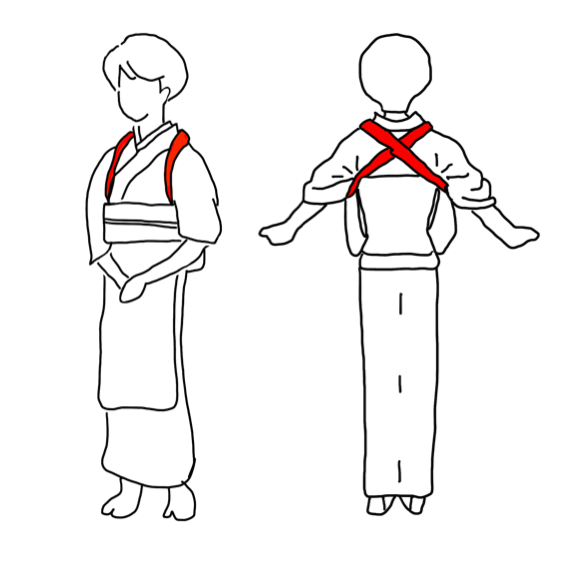
\includegraphics[width=0.25\textwidth]{./figures/tasuki-gake01.png}
    \caption{襷掛け: 和服の袂が作業をする際に邪魔になるので、長い布紐で、背中がクロスになるように袂を手繰り寄せる肩紐の掛け方。}\label{fig:tasuki-gake-picture-j}
  \end{figure}
\else
  \begin{figure}[htb]\centering\small
    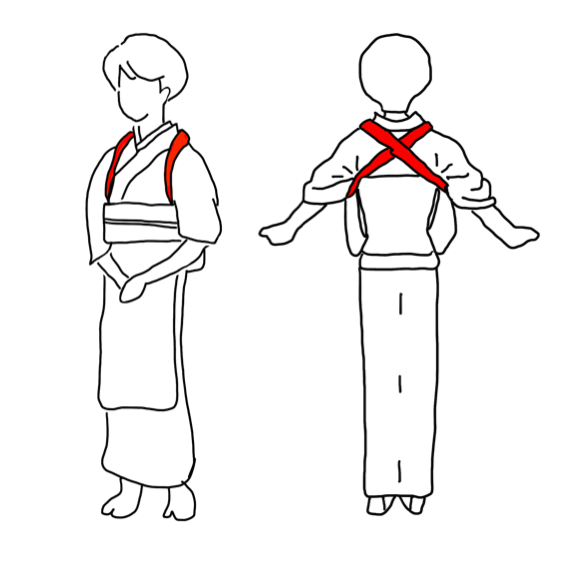
\includegraphics[width=0.25\textwidth]{./figures/tasuki-gake01.png}
    \caption{Tasuki-gake: a method of tying a long cloth strap around the back to pull the sleeves of a kimono together, so that they cross over the back. This is done to prevent the sleeves from getting in the way while working.}\label{fig:tasuki-gake-picture}
  \end{figure}
\fi

\ifJPN
  \begin{figure}[htb]\centering\small
    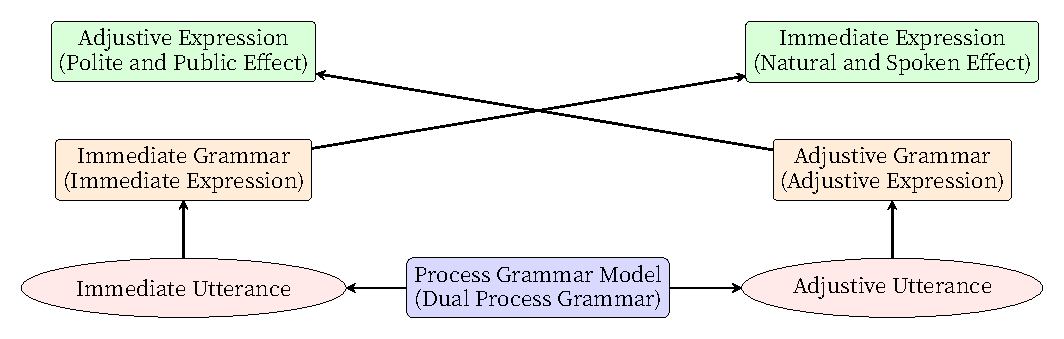
\includegraphics[width=0.95\textwidth]{tasuki-gake.pdf}
    \caption{襷掛け効果: プロセス文法における効果の交差的構造。
    日本の伝統的な「たすき掛け」は、前と後ろで左右の紐が交差する形式をとる。これは、即時的な発話が調整的効果を、調整された発話が自然で親しみやすい印象を生むという、効果と使用の関係の「ねじれ」を視覚的に表す比喩である。
    }\label{fig:tasuki-gake-j}
  \end{figure}
\else
  \begin{figure}[htb]\centering\small
    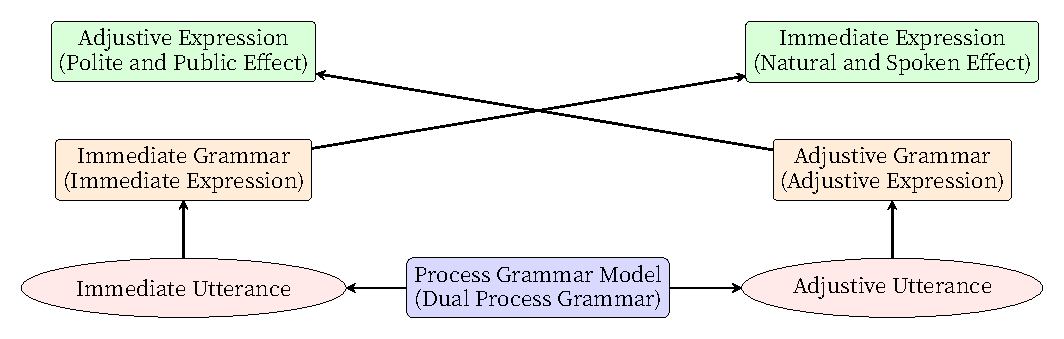
\includegraphics[width=0.95\textwidth]{tasuki-gake.pdf}
    \caption{Tasuki-gake Effect: A Visual Metaphor for Crossed Effects in Process Grammar. The diagram illustrates the traditional way of tying a tasuki sash. Just as the front-left is tied to the back-right, and vice versa, the relationship between utterance types and their perceived effects often crosses over. Immediate utterances can produce polite effects, while adjusted utterances may evoke natural or spontaneous impressions.
    }\label{fig:tasuki-gake}
  \end{figure}
\fi

\ifJPN
本モデルでは、言語の使用はまず時間的基盤において二種の発話(utterance)に分けられる。すなわち、即時に発せられる「Immediate Utterance(即時発話)」と、熟考や調整の後に発せられる「Adjustive Utterance(漸次発話)」である。
この二種の発話は、それぞれ異なる文法的拘束を受ける。Immediate Utterance は直感的な発話の連鎖を導く「Immediate Grammar(即時文法)」に支えられ、Adjustive Utterance は判断や推敲を経た表現の形成を担う「Adjustive Grammar(調整文法)」に支えられる。

ここから生まれる言語表現は、それぞれ「Immediate Expression(即時表現)」「Adjustive Expression(調整表現)」と呼ばれるが、重要なのは、それらの表現が使用される状況によって逆方向の効果を持ち得るという点である。
Adjustive Expression が訓練や定型化を経て即時に発話されたとき、それは公的かつ丁寧な印象を与える「Polite and Public Effect(丁寧・公的効果)」をもたらす。
一方、Immediate Expression が意図的に小説やインタビュー記事などに組み込まれた場合には、生き生きとした会話的な印象を与える「Natural and Spoken Effect(自然・話しことば的効果)」を発揮する。

このように、発話の時間的性質と、表現の出自が生む効果の間には交差関係(襷掛け)が存在しており、単純な二分法では捉えきれない表現の機能と運用の豊かさを可視化する構造となっている
(図 \ref{fig:tasuki-gake-picture-j}, \ref{fig:tasuki-gake-j})。

\else

In this model, language use is fundamentally categorized by two temporal types of utterance:
Immediate Utterance, which is produced spontaneously in real time, and
Adjustive Utterance, which is the result of thoughtful planning and adjustment.
Each type of utterance is governed by a distinct grammatical system.
Immediate Utterance operates under Immediate Grammar, which facilitates intuitive and real-time chaining of expressions.
Adjustive Utterance, in contrast, is governed by Adjustive Grammar, which supports expressions formed through careful deliberation and revision.

The expressions derived from these grammars are referred to as
Immediate Expression and Adjustive Expression, respectively.
However, a crucial feature of this model is that these expressions can produce cross-directional effects depending on how they are used.
When an Adjustive Expression is highly practiced, formulaic, or trained for immediate delivery,
it gives rise to the Polite and Public Effect, creating a sense of formality, refinement, or social appropriateness.
Conversely, when an Immediate Expression is intentionally employed in written or scripted media—such as novels or interviews...
    it produces the Natural and Spoken Effect, evoking a vivid, conversational, and lifelike tone.

Thus, there is a crossed (tasuki-gake) relationship between the temporal nature of utterance and the effect of expression.
This structure makes visible the richness of expressive function and practical use that goes beyond a simple binary model.(Figure \ref{fig:tasuki-gake-picture} and \ref{fig:tasuki-gake}).
\fi

\ifJPN
\section{記述の方法}
\else
\section{Description Method}
\fi

\ifJPN
\subsection{適切なフォーマットの設計}
\else
\subsection{Design of Appropriate Format}
\fi

\ifJPN
即時文法と調整文法を関係づける際には、それぞれが担う役割を反映したフォーマットをデザインする。
このフォーマットでは、各プロセスがどのタイミングでどのように発動するかを示す「プロセスのフロー」を明確に示す。
たとえば、即時文法では「反応的発話」の発生時点を明記し、その後に調整文法が適用される「修正」や「確認」のタイミングを示すことによって、異なるフォーマットを維持しつつ、両者の補完を視覚的に表現できる。
\else
When linking immediate grammar and adjustive grammar, design a format that reflects the roles they play.
In this format, clearly show the ``flow of processes'' that indicates when and how each process is triggered.
For example, in immediate grammar, clearly indicate the timing of the occurrence of ``reactive speech,'' and by indicating the timing of ``correction'' and ``confirmation'' to be applied later, it is possible to visually express the complementarity of the two while maintaining different formats.
\fi

\ifJPN
\subsection{区別のメタレベルでの検討}
\else
\subsection{Consideration at the Meta-level of Distinction}
\fi
  
\ifJPN
即時文法と調整文法は一見するとつながっているように見えるかもしれないが、実はそれぞれが異なる認知的・社会的な機能を持つ。
この点において両者が異なる状況や認知負荷の下で機能するかどうかを観察することが課題である。
たとえば、即時文法が「認知的な即時反応」を、調整文法が「複雑な言語調整を伴う認知過程」を反映しているならば、それぞれの理論的枠組みを区別するロジックが自ずと確立できよう。
\else
Although immediate grammar and adjustive grammar may seem to be connected at first glance, they actually have different cognitive and social functions.
It is a challenge to observe whether they function under different situations and cognitive loads.
For example, if immediate grammar reflects ``cognitive immediate responses'' and adjustive grammar reflects ``cognitive processes involving complex language adjustments,'' the logic to distinguish between the two theoretical frameworks will naturally be established.
\fi

\ifJPN
\subsection{実証的データによる区別の確認}
\else
\subsection{Confirmation of Distinction by Empirical Data}
\fi

\ifJPN
理論を実証的に支えるデータを集める目的は、即時文法と調整文法が異なる文脈や使用場面での具体的な発話例からシステムを構築することである。
即時文法と調整文法の両者の特徴を実例で、実際に次元分けしたマップ上にピン止めするなどして固定し、概念化の助けにすることで両極が実在性することを示し、その上にプロセス文法が横たわっていることを示す。
実際の会話や言語データを分析し、即時的な反応と時間を要する調整の区別、またはそれらのタイミングにより、両極が曖昧になるのかどうかを確認することで、具体的に両極を整理する。
\else
The purpose of collecting data to empirically support the theory is to build a system from specific speech examples in different contexts and usage situations of immediate grammar and adjustive grammar.
By pinning down the characteristics of both immediate grammar and adjustive grammar on a map divided into dimensions with actual examples, it is possible to show that both poles exist and that the process grammar lies on top of them.
By analyzing actual conversations and language data, it is possible to confirm whether the distinction between immediate responses and time-consuming adjustments, or the timing of these, makes the two poles ambiguous, and to organize them concretely.
\fi

\ifJPN
関係づける方法としては、即時文法のフォーマットにおける「反応的な要素」を調整文法のフォーマットにおける「調整過程」とのリンクの方法を提案することが一つのアプローチになる。
両極を取り持つ実際的なデータをモデルとして位置付けることで、言語の使用における「即時性」と「調整性」が相互作用するモデルのパラメタを指定できれば、相対的な発話・表現の連続体モデルが作成できると考える。
\else
One approach is to propose a method of linking the ``reactive elements'' in the format of immediate grammar with the ``adjustment process'' in the format of adjustive grammar.
By positioning actual data that mediates both poles as a model, it is possible to specify the parameters of a model in which ``immediacy'' and ``adjustability'' in language use interact, and to create a model of a continuum of relative speech and expressions.
\fi

%- 両極の特徴を説明。
%  - 即時文法の特徴: 緊急性、直感的反応(例: 「危ない!」)。
%  - 調整文法の特徴: 慎重な推敲、フォーマルな場面での使用(例: スピーチ)。
%- 中間的な状況やグラデーションを含めたモデルを提案。
%  - 日常会話の中での即時的発話と調整的発話の組み合わせ。
%  - 例えば、初対面の相手への対応では即時性と調整性が同時に求められる。
%- 視覚化(図や表)を活用。
%  - モデルのグラフやフローチャート。
%  - 即時性から調整性への連続体を示す視覚的表現。


% 補足の提案
% 
% 1. 定義の明確化  
%    「調整」が形式に限定されることを強調する際、具体的な例を挙げると読者の理解が深まります(例: 丁寧表現の選択、文法的再構成)。
% 
% 2. 視覚化の内容を事前に予告
%    視覚化が含まれることは非常に良いですが、図や表の具体的な形式(連続体のスペクトラムや事例比較表など)を明記すると、期待感が高まります。
% 
% 3. 各セクションの間のつながり
%    「定義」と「モデル」のセクションが緊密に関連していることを示すために、「モデル提案」が定義を基に構築されている旨を冒頭で簡単に述べるのが効果的です。


% \begin{figure}[ht]\centering
%     \includegraphics[width=0.7\textwidth]{processimage.pdf}
%     \caption{
%       Process grammar model of actual language use: 
%       continuum of immediate and adjusted grammars
%     }
%     \label{fig:processgrammar}
% \end{figure}

\begin{figure*}[ht]\centering\small
\begin{tikzpicture}[scale=.8, every node/.style={align=center, font=\small}]
\draw[thick] (0,0) rectangle (10,4);
\draw[thick, dashed] (0,0) -- (10,4);
\fill[blue!20, opacity=0.6] (0,0) -- (10,4) -- (0,4) -- cycle; % Upper triangle for 即時文法
\fill[red!20, opacity=0.6] (0,0) -- (10,4) -- (10,0) -- cycle; % Lower triangle for 調整文法
\ifJPN
  \node[above left] at (4,2.5) {即時文法};
  \node[below right] at (6,1.5) {調整文法};
  \node[above right] at (4,1.6) {連続体};
  \node[above left] at (0,1.5) {高い\\即時性};
  \node[below right] at (10,2.5) {高い\\調整性};
\else
  \node[above left] at (4.2,2.5) {Immediate Grammar};
  \node[below right] at (6,1.5) {Adjustive Grammar};
  \node[above right] at (3.5,1.6) {Continuum};
  \node[above left] at (0,1.5) {High\\Immediacy};
  \node[below right] at (10,2.5) {High\\Adjustability};
\fi
\end{tikzpicture}

\ifJPN
\caption{実際の言語使用のプロセス文法モデル:即時性と調整性の連続体}
\else
\caption{Process grammar model of actual language use}
\fi

\label{fig:processgrammar}
\end{figure*}

\ifJPN
\begin{table*}[ht]\centering\small
\caption{即時文法と調整文法の特徴}
\else
\begin{table*}[ht]\centering\small
\caption{Characteristics of immediate and adjustment grammars}
\fi
\label{tab:characteristics}
\ifJPN
\begin{tabular}{lp{4.5cm}p{8.5cm}}\noalign{\hrule height .8pt}
\textbf{項目} 
  & \textbf{即時文法}
  & \textbf{調整文法} \\ \hline

\textbf{特徴} 
  & その場で瞬間的に適用される文法。
  & 言語形式が適切かを検討し、必要に応じて修正・調整を行う文法。 \\ 

\textbf{時間幅} 
  & ミリ秒から数秒で処理される。 
  & 数秒から数年まで、長い時間をかけて調整される場合もある。 \\ 

\textbf{具体例} 
  & 反射的な応答、自然発生的な会話。 
  & 記者会見の応答(調整を伴う場合)、スピーチ、法律文書の推敲。 \\ 

\textbf{調整の要素} 
  & 微小の調整、無意識的な調整のみ。 
  & 言語形式に関する意識的な調整が加えられる。 \\ 

\textbf{目的} 
  & 即座に情報を伝える。 
  & 誤解を防ぎ、正確性や適切さを確保する。 \\
\end{tabular}
\end{table*}

\else

  \begin{tabular}{p{32mm}p{53mm}p{60mm}}\noalign{\hrule height .8pt}
%  & \textbf{Immediate Grammar} & \textbf{Adjustment Grammar} \\

  \textbf{Item} 
  & \textbf{Immediate Grammar} 
  & \textbf{Adjustive Grammar} \\ \hline

  \textbf{Characteristics} 
  & Grammar applied instantaneously on the spot. Little consideration or modification of form. 
  & Grammar that considers the appropriateness of linguistic forms and makes adjustments as needed. \\

  \textbf{Time Span} 
  & Milliseconds to seconds. Processed in real-time. 
  & Seconds to years. Adjustments may take a long time. \\

  \textbf{Examples} 
  & Reflexive responses, spontaneous conversations. 
  & Press conference responses (with adjustments), speeches, editing of legal documents. \\

  \textbf{Adjustive Elements} 
  & Minimal or unconscious adjustments only. 
  & Conscious adjustments to linguistic forms. \\

  \textbf{Purpose} 
  & Immediate information delivery. 
  & Preventing misunderstandings and ensuring accuracy and appropriateness. \\
\end{tabular}
\end{table*}
\fi





\ifJPN
  \section{今後の展開}
\else
  \section{Future Directions}
\fi

\ifJPN
  \subsection{研究課題}
\else
  \subsection{Research Questions}
\fi

\begin{itemize}
  \item 
\ifJPN
即時文法と調整文法の境界とその定式化(前限界・後限界の数式化)
\else
The boundary between Immediate Grammar and Adjustive Grammar and its formalization (formulation of pre-boundary and post-boundary)
\fi

  \item 
\ifJPN
実証データの収集と分析(会話データ、書きことばデータの比較)
\else
Collection and analysis of empirical data (comparison of conversation data and written data)
\fi
\end{itemize}

\ifJPN
  \subsection{アップデートの方針}
\else
  \subsection{Update Policy}
\fi

\ifJPN
ルールベースの整理と追加
\else
Organizing and adding rules
\fi
\ifJPN
言語教育やAI(自然言語処理)への応用
\else
Application to language education and AI (natural language processing)
\fi
\ifJPN
和歌や歴史的な文献を対象にした分析を検討していく。
\else
Consideration of analysis targeting waka and historical literature.
\fi

\ifJPN
  \section{おわりに}
\else
  \section{Conclusion}
\fi

\ifJPN
本ダイジェストでは、プロセス文法モデルの概要、即時文法と調整文法の対比、理論的背景を示した。今後のアップデートでは、ルールベースの整理やデータ分析を拡充し、さらなる発展を目指す。
\else
In this digest, we have outlined the Process Grammar Model, compared Immediate Grammar and Adjustive Grammar, and discussed the theoretical background. In future updates, we will expand the rule base and data analysis to further develop the model.
\fi

\appendix
\ifJPN
\section{Q\&A セクションについて}
\else
\section{About the Q\&A Section}
\fi
\label{sec:QandA}

\ifJPN
本書では、即時文法の理論モデルを提示し、それに基づく実例や応用を通じて新たな言語理解の枠組みを探ってきた。しかし、こうした新しい理論を提示するにあたっては、読者の視点からさまざまな疑問や確認したい点が生まれることも予想される。
\else
In this book, we have presented the theoretical model of immediate grammar and explored a new framework for language understanding through examples and applications based on it. However, when introducing such a new theory, it is expected that various questions and points of confirmation will arise from the reader's perspective.
\fi

\ifJPN
この「Q\&A セクション」では、そうした疑問に対する著者の立場や補足的な考察を記録しておくことを目的とする。また、このセクションには、翻訳作業(たとえば『土佐日記』『伊勢物語』)や、日々の即時文法表現の収集作業(aeadプロジェクト)において、思考の過程で浮かび上がった疑問や発見も含めていく。
\else
This ``Q\&A Section'' aims to record the author's position and supplementary considerations regarding such questions. Additionally, this section will include questions and discoveries that have emerged during the translation work (for example, ``Tosa Nikki'' and ``Ise Monogatari'') and the daily collection of immediate grammar expressions (aead project).
\fi

\ifJPN
本文に組み込むには構成上の調整が必要となるが、それとは別に「書くたびに微妙なズレが生じる」ことを避け、思考のまとまりを維持するために、このセクションを用いる。必要に応じて本文との連携を後から再検討することを想定しており、本セクションは柔軟な蓄積と検討の場として位置づけられている。
\else
To avoid ``subtle discrepancies that arise every time I write'' and to maintain the coherence of thought, this section will be used. It is assumed that the integration with the main text will be reconsidered later as needed, and this section is positioned as a flexible space for accumulation and examination.
\fi

\ifJPN
\subsection{Q\&A: 即時文法とその理論的背景}
\else
\subsection{Q\&A: Immediate Grammar and Its Theoretical Background}
\fi

% 連番Q&A:最初のグループ
\begin{enumerate}[label=\textbf{Q\arabic*.}, leftmargin=2em]

  \item \label{qa:20250405a}
\ifJPN
  \textbf{即時文法とはどのような理論ですか? また、既存の構文理論とどのように位置づけられるのですか?}
\else
  \textbf{What kind of theory is Immediate Grammar? How is it positioned in relation to existing syntactic theories?}
\fi

\ifJPN
  \textbf{A.} 即時文法は、言語使用に見られる即時的かつ柔軟な表現形式に注目し、それらを理論的に説明しうる構造として提案されるものです。このモデルは、句構造文法のような構文中心の理論と対置されるものではなく、同等の立場において、人間の言語行動を異なる観点から記述しようとする仮説的枠組みです。
\else
  \textbf{A.} Immediate Grammar focuses on the immediate and flexible forms of expression observed in language use and proposes them as structures that can be theoretically explained. This model is not positioned in opposition to syntactic-centered theories like phrase structure grammar but is a hypothetical framework that aims to describe human language behavior from a different perspective.
\fi

  \item \label{qa:20250405b}
\ifJPN
  \textbf{即時文法は、どのような点で言語記述に貢献するのですか?}
\else
  \textbf{In what ways does Immediate Grammar contribute to language description?}
\fi

\ifJPN
  \textbf{A.} 即時文法という視点を導入することで、これまで「例外的」または「構造に乏しい」とされてきた発話が、体系的な言語使用の一形態として位置づけられるようになります。これは、即時文法がそうした発話に対して理論的な「説明のスロット」を提供するモデルであることの証とも言えます。
\else
  \textbf{A.} By introducing the perspective of Immediate Grammar, utterances that have previously been considered "exceptional" or "lacking structure" can be positioned as a systematic form of language use. This can be seen as evidence that Immediate Grammar provides a theoretical "slot for explanation" for such utterances.
\fi

\end{enumerate}

\ifJPN
\section{用例と実践からの考察}
\else
  \section{Considerations from Examples and Practice}
\fi

\begin{enumerate}[resume, label=\textbf{Q\arabic*.}, leftmargin=2em]

  \item \label{qa:20250406a}
\ifJPN
  \textbf{即時文法は話しことばと同じですか?}
\else
  \textbf{Is Immediate Grammar the same as spoken language?}
\fi

\ifJPN
  \textbf{A.} 即時文法は「話しことば」と混同されがちですが、理論的には異なる概念です。即時文法は、心理的処理のタイミングや構造の柔軟性を基準とした文法モデルであり、口頭表現であっても調整文法が用いられることもあります。
\else
  \textbf{A.} Immediate Grammar is often confused with "spoken language," but theoretically, they are different concepts. Immediate Grammar is a grammatical model based on the timing of psychological processing and structural flexibility, and even in oral expressions, adjusted grammar can be used.
\fi

  \item \label{qa:20250406b}
\ifJPN
  \textbf{Q\&A: なぜコーパスを用いた自動抽出を行わないのですか?}
\else
  \textbf{Q\&A: Why don't you use corpus-based automatic extraction?}
\fi

\ifJPN
  \textbf{A.} 近年の言語研究では、構文のパターンをコーパスから一括して抽出する方法が広く用いられています。これは形式的な構造(語順・係り受け・品詞パターン)に関する分析にとって非常に有効な手法です。
しかし、即時文法が対象とするのは、単なる構文のかたちではなく、「発話の仕方」「反応の仕方」「その瞬間に選択された表現」そのものであり、これは構文的なラベルや構造情報だけでは判断できません。 
たとえば、「そうそう、それそれ」といった発話や、「うん、でもさあ」のような連続表現は、文法的に曖昧で断片的に見えるかもしれませんが、即時的な判断・感情・反応の流れに基づく高度な構造を持っています。
こうした現象は、コーパス中にあっても、「検索条件に合致しない」「文法的なまとまりとして認識されない」といった理由で取りこぼされやすく、むしろ人間の目による文脈的判断と、経験に基づく記述的作業のほうが正確に取り扱えると考えています。
したがって、本研究では、既存のコーパスベースの方法と対立するのではなく、補完的なものとして、記述と言語直観に基づく観察的アプローチを採用しています。
\else
  \textbf{A.} In recent language research, methods for extracting syntactic patterns from corpora have been widely used. This is a very effective method for analyzing formal structures (word order, dependency, part-of-speech patterns).
However, what Immediate Grammar targets is not just the form of syntax but the "way of speaking," "way of responding," and "expressions chosen at that moment," which cannot be judged solely by syntactic labels or structural information.
For example, utterances like "そうそう、それそれ" (yes, yes, that's it) or continuous expressions like "うん、でもさあ" (yeah, but you know) may seem grammatically ambiguous and fragmented, but they have a sophisticated structure based on immediate judgments, emotions, and the flow of responses.
Such phenomena, even if present in the corpus, are often overlooked due to reasons like "not matching search criteria" or "not recognized as grammatical coherence," and it is believed that they can be more accurately handled through contextual judgment by human eyes and descriptive work based on experience.
Therefore, in this study, we adopt an observational approach based on description and linguistic intuition, not in opposition to existing corpus-based methods but as a complementary one.
\fi

\item \label{qa:20250405d}
\ifJPN
  \textbf{Q\&A: 即時文法は、会話分析やディスコース分析のような録音・文字化・分析の手続きを無視しているのですか?}
\else
  \textbf{Q\&A: Does Immediate Grammar ignore the procedures of recording, transcription, and analysis like conversation analysis or discourse analysis?}
\fi

\ifJPN
  \textbf{A.} いいえ、本研究における即時文法の立場は、ディスコース分析や会話分析が対象とする「発話の具体性」や「文脈への依存性」と共通する部分を多く持っています。特に、文脈に応じた語の選択、タイミング、相づち、言い直しなどの発話の連続性は、即時文法の重要な観察対象でもあります。
ただし、分析手法としては異なります。会話分析やディスコース分析では、音声の録音→文字化→発話単位の構造分析という手続きを通じて、参加者間の相互行為を記述します。これに対して、即時文法の目的は、こうした発話に見られるパターンを、発話者が瞬時に選択・操作している構造のモデルとして記述することです。
そのため、本研究では、録音・文字化という手続き自体は採用していませんが、それを前提にした発話資料や用例を十分に参照しており、観察の焦点が「使用されている即時的構造」にあるという点で、補完的なアプローチをとっています。
要するに、即時文法は、ディスコース分析や会話分析の成果と矛盾するものではなく、それらが描き出した「細かな発話現象」の背景にある構造的説明モデルとして機能することを目指しているのです。
\else
  \textbf{A.} No, the position of Immediate Grammar in this study shares many commonalities with the "specificity of utterances" and "contextual dependence" targeted by discourse analysis and conversation analysis. In particular, the continuity of utterances, such as word choice according to context, timing, backchanneling, and rephrasing, is also an important observation target of Immediate Grammar.
However, the analytical methods differ. In conversation analysis and discourse analysis, the procedure of recording audio → transcribing → structural analysis of utterance units is used to describe the interaction between participants. In contrast, the purpose of Immediate Grammar is to describe the patterns observed in such utterances as a model of the structures that speakers instantaneously select and manipulate.
Therefore, while this study does not adopt the procedures of recording and transcription, it sufficiently references utterance materials and examples based on them, taking a complementary approach in that the focus of observation is on the "immediate structures being used."
In short, Immediate Grammar does not contradict the results of discourse analysis or conversation analysis; rather, it aims to function as a structural explanatory model underlying the "detailed utterance phenomena" they depict.
\fi


\item \label{qa:20250413a}
\ifJPN
  \textbf{「継ぎ足し構文」や「連節文法」は、即時文法とどのような関係がありますか?}
\else
  \textbf{How are chaining constructions or chaining grammar related to Immediate Grammar?}
\fi

\ifJPN
  \textbf{A.} 「継ぎ足し構文」や「連節文法」は、複雑な文構造を動的かつ直感的に組み立てる際によく見られる形式であり、即時文法の重要な具体例の一つです。たとえば、話しながら順次内容を加えていく「〜て」「〜で」「〜けど」などの文は、文の全体像を事前に設計せずに生成される点で、即時文法の本質を示しています。このような文は、語りの流れに従って言語を構築していく人間の行動に密接に対応します。
\else
  \textbf{A.} Chaining constructions or chaining grammar represent a common form used when constructing complex sentences in a dynamic and intuitive way. They are a key manifestation of Immediate Grammar. For instance, sentences formed with expressions like “and then,” “but,” or “so,” which are added successively as one speaks, exemplify the nature of Immediate Grammar, as they are generated without pre-planning the entire sentence. These forms closely correspond to how people construct language in real-time.
\fi


\item \label{qa:20250413b}
\ifJPN
  \textbf{外国語話者にとって、「の」を使った修飾より「で」や「て」で継ぎ足す構文の方が自然に使えるのはなぜですか?}
\else
  \textbf{Why is it easier for non-native speakers to use constructions with "de" or "te" rather than complex noun phrases with "no"?}
\fi

\ifJPN
  \textbf{A.} 「の」を用いた修飾構文は、名詞の前に長い形容語句を積み重ねる必要があり、文全体を構造的に計画する調整文法的処理を求められます。これに対し、「で」や「て」などを使って行為や情報を順に継ぎ足していく構文は、出来事や行為の流れに沿って逐次的に発話できるため、即時文法的です。たとえば、「昨日駅で見た赤い帽子の女の子」は、「赤い帽子の女の子」が長く修飾された名詞であり、語順や係り受けが複雑になります。一方で、「昨日、駅に行って、赤い帽子をかぶった女の子を見た」という表現は、順を追って構成され、文としての完成を逐次先送りできるため、初級者にも自然で扱いやすい形式となります。これは英語でも同様で、``the girl who wore a red hat that I saw at the station yesterday'' よりも、``I went to the station yesterday and saw a girl. She was wearing a red hat.'' の方が習得が容易であることと対応しています。
\else
  \textbf{A.} Japanese constructions using ``no'' require stacking modifiers in front of a noun, which demands structural planning and is characteristic of Adjustive Grammar. In contrast, constructions using ``de'' or ``"te'' allow for sequential chaining of events or states, enabling spontaneous, step-by-step utterance—hallmarks of Immediate Grammar. For instance, the phrase "kinō eki de mita akai bōshi no onna no ko'' (``the girl in the red hat I saw at the station yesterday'') involves a complex noun phrase with multiple layers of modification. Meanwhile, a sentence like ``"Kinō eki ni itte, akai bōshi o kabutta onna no ko o mita" (``I went to the station yesterday and saw a girl wearing a red hat'') follows a chronological flow and allows the speaker to build the sentence incrementally. This is similar in English: ``The girl who wore a red hat that I saw at the station yesterday'' is structurally demanding, while ``I went to the station yesterday and saw a girl. She was wearing a red hat.'' is easier to produce and understand, especially for language learners.
\fi
\end{enumerate}

\ifJPN
\section{即時文法の事例集}
\else
\section{Examples of Immediate Grammar}
\fi
\label{sec:immediate_grammar_examples}

\ifJPN
\subsection{即時文法の実在性を支える観察の蓄積}
\else
\subsection{Accumulation of Observations Supporting the Existence of Immediate Grammar} 
\fi
\label{subsec:immediate_grammar_observations}

\ifJPN
本書では、「即時文法」という理論枠組みを提示しているが、その背景には、著者自身が行ってきた複数の実践的観察と記録がある。たとえば、『伊勢物語』や『土佐日記』の翻訳において、表現の自然な現代語訳を模索する過程で、従来の構文理論では説明が困難な即時的表現が多く見出された。また、aead(An expression a day)プロジェクトにおいては、日常的な日本語表現の中に即時文法の特徴を持つ表現を日々記録し、それらにタグと注釈を加えることで、言語使用の実態と即時文法の対応を浮かび上がらせてきた。
\else
In this book, we present the theoretical framework of "Immediate Grammar," which is supported by multiple practical observations and records made by the author. For example, in the process of translating works like "Ise Monogatari" and "Tosa Nikki," many immediate expressions were found that are difficult to explain using conventional syntactic theories. Additionally, in the aead (An expression a day) project, we have been recording expressions with characteristics of immediate grammar in everyday Japanese, tagging them, and adding annotations to highlight the correspondence between language use and immediate grammar.
\fi

\ifJPN
これらの作業は、直観的な主張ではなく、時間をかけて蓄積された観察の成果である。数百に及ぶ用例が、それぞれ即時文法の視点から解釈・記述されており、結果として、即時文法という理論が記述モデルとして有効であることを示す実証的な手がかりとなっている。
\else
These tasks are not based on intuitive claims but are the results of observations accumulated over time. Hundreds of examples have been interpreted and described from the perspective of immediate grammar, providing empirical clues that demonstrate the effectiveness of immediate grammar as a descriptive model.
\fi

%\subsection{土佐日記「よねさけ、しばしばくる」の語順と焦点化} \label{ex:yonosake}

%\subsection{伊勢物語「それがこうなる」の指示と文脈依存性} \label{ex:soregakounaru}

%\subsection{即時文法における「て連鎖」の認知処理} \label{ex:te-rensa}

% grammar-as-performance.tex

\ifJPN
\section{文法と演出:語りの構造と即時文法}
\else
\section{Grammar and Performance: The Structure of Narration and Immediate Grammar}
\fi

\ifJPN
従来の言語学において、語りの「演出効果」が文法構造によって直接的に支えられているという視点は、必ずしも体系的に扱われてこなかった。生成文法は意味と構造に、語用論は話し手の意図に焦点を当ててきたが、語りにおける構文の選択が、即時的な演出(surprise, reveal, buildup)の効果をどのように生成しうるかについては、部分的な言及にとどまっている。
\else
In traditional linguistics, the perspective that the "performance effect" of narration is directly supported by grammatical structure has not been systematically addressed. Generative grammar has focused on meaning and structure, while pragmatics has concentrated on the speaker's intention. However, there has been only partial mention of how the choice of syntax in narration can generate immediate performance effects (surprise, reveal, buildup).
\fi

\ifJPN
プロセス文法モデル(PGM)では、文法は単なる意味構築の枠組みにとどまらず、語り手が聞き手の注意・感情・予測を制御する「演出の構造」として機能することを前提とする。特に即時文法においては、語り手がその場で思い浮かべた順序で情報を提示する際に、主語の遅延や場所句の先行、動作句の先行挿入などがしばしば現れる。これらの構造は、認知的処理における「舞台設定→drum-roll→焦点開示」という演出的効果を持ち、構文そのものがその効果を支えている。
\else
In the Process Grammar Model (PGM), grammar is not merely a framework for meaning construction but functions as a "structure of performance" that allows the narrator to control the listener's attention, emotions, and predictions. In particular, in immediate grammar, when the narrator presents information in the order they think of it on the spot, structures such as subject delay, preposing of locative phrases, and insertion of action phrases often occur. These structures have a performative effect of "setting the stage → drum-roll → focus disclosure" in cognitive processing, and the syntax itself supports that effect.
\fi

\ifJPN
たとえば、「山の中から、出てきた出てきた、羊さんたちでーす」という語りは、「場所→動詞句→主語」という語順であり、英語の Locative Inversion(From the box came a bird.)と構造的に一致する。しかしこの語順は、即時的に生成された語りの流れであり、調整された表現の即時使用による襷掛け効果ではなく、即時文法の内在的構文である。
\else
For example, the narration "From the mountains, here come the sheep!" follows the order "locative → verb phrase → subject," structurally matching English Locative Inversion (From the box came a bird.). However, this word order is part of an immediately generated narrative flow and is not an effect of immediate use of adjusted expressions; it is an intrinsic syntax of immediate grammar.
\fi

\ifJPN
このような例においては、演出は文法に従属するのではなく、むしろ文法が演出を可能にする枠組みそのものとなっている。よって、PGMにおける「文法と演出」の関係は、構文選択の動機が「意味」だけでなく「効果(エフェクト)」にあることを明示する必要がある。
\else
In such examples, the performance does not depend on grammar; rather, grammar itself becomes the framework that enables the performance. Therefore, in PGM, the relationship between "grammar and performance" needs to clarify that the motivation for syntactic choice lies not only in "meaning" but also in "effect."
\fi


\if0
\ifJPN
\subsection*{今後の課題}
\else
\subsection*{Future Tasks}
\fi

\begin{itemize}
  \ifJPN
  \item AEAD における即時表現のうち、「焦点遅延」や「出現語順(場所→動作→主語)」が用いられている事例の収集と分類。
  \item 『伊勢物語』『土佐日記』の語りにおける即時的演出構造の記述と、和文構文との対応の明確化。
  \item BibLaTeX を用いた文献注の構築。以下の文献は本節に関連する基本資料である。

  \else

  \item Collection and classification of instances in AEAD where immediate expressions such as "focus delay" and "emergent word order (locative → action → subject)" are used.
  \item Description of immediate performance structures in the narration of "Ise Monogatari" and "Tosa Nikki," and clarification of their correspondence with Japanese syntax.
  \item Construction of bibliographic notes using BibLaTeX. The following references are basic materials related to this section:

\fi

  \begin{itemize}
      \item Birner, B. J. (1996). \textit{The Discourse Function of Inversion in English}. Garland Publishing.
      \item Huddleston, R., \& Pullum, G. K. (2002). \textit{The Cambridge Grammar of the English Language}. Cambridge University Press.
      \item Ward, G., \& Birner, B. J. (1995). Definiteness and the English Existential Construction. \textit{Language}, 71(4), 722–742.
      \item Quirk, R. et al. (1985). \textit{A Comprehensive Grammar of the English Language}. Longman.
    \end{itemize}
\end{itemize}
\fi


\printbibliography
\end{document}
